Die experimentellen Daten werden anhand der aufgezeichneten Messwerte systematisch ausgewertet. Hierbei werden die maximale Scherkraft, die durchschnittliche Scherkraft sowie die Bruchfläche der Prüfkörper für beide Fertigungsverfahren, Laminierung und Sintern, berechnet. Die ermittelten Werte werden in tabellarischer Form dargestellt und hinsichtlich ihrer Abweichungen analysiert. (siehe \hyperref[Tab.1]{Tabelle 1} und \hyperref[Tab.2]{Tabelle 2})
Die Scherfestigkeit wird nach folgender Formel bestimmt:
\begin{equation}
    \sigma_{\text{Scher}} = \frac{F_{\text{max}}}{A} \quad \text{mit } F_{\text{max}} \text{ in } \si{\newton}, A \text{ in } \si{\milli\meter\squared}
\end{equation}

\begin{table}[H]
\centering

\adjustbox{max width=\textwidth}{

% Resize the table to fit within the page
%\resizebox{\textwidth}{!}{%


\renewcommand{\arraystretch}{1.7} % Increase row height (local)
\fontsize{18pt}{20pt}\selectfont
\begin{tabular}{|l|c|c|c|c|}
\hline
\textbf{Scherkörper} & \multicolumn{1}{l|}{\textbf{Maximale Scherkraft} {[}\si{\newton}{]}} & \multicolumn{1}{l|}{\textbf{Durchschnittskraft} {[}\si{\newton}{]}} & \multicolumn{1}{l|}{\textbf{Fläche} {[}\si{\milli\meter\squared}{]}} & \multicolumn{1}{l|}{\textbf{Scherfestigkeit} {[}\si{\newton\per\milli\meter\squared}{]}} \\ \hline
\textbf{1} & 330,45 & 143,11 & 5,29 & 62,47 \\ \hline
\textbf{2} & 459,23 & 137,78 & 5,29 & 86,81 \\ \hline
\textbf{3} & 420,47 & 135,23 & 5,29 & 79,48 \\ \hline
\textbf{4} & 384,35 & 148,57 & 5,29 & 72,66 \\ \hline
\textbf{5} & 508,97 & 172,81 & 5,29 & 96,21 \\ \hline
\textbf{6} & 358,84 & 116,34 & 5,29 & 67,83 \\ \hline
\textbf{7} & 388,41 & 143,01 & 5,29 & 73,42 \\ \hline
\textbf{8} & 354,98 & 140,97 & 5,29 & 67,10 \\ \hline
\end{tabular}}
\vspace{0.5cm}
\caption{Messung der gesinterten Scherkörper}
\label{Tab.1}
\end{table}




\begin{table}[H]
\centering

\adjustbox{max width=\textwidth}{

% Resize the table to fit within the page
%\resizebox{\textwidth}{!}{%


\renewcommand{\arraystretch}{1.7} % Increase row height (local)
\fontsize{18pt}{20pt}\selectfont
\begin{tabular}{|l|c|c|c|c|}
\hline
\textbf{Scherkörper} & \multicolumn{1}{l|}{\textbf{Maximale Scherkraft} {[}\si{\newton}{]}} & \multicolumn{1}{l|}{\textbf{Durchschnittskraft} {[}\si{\newton}{]}} & \multicolumn{1}{l|}{\textbf{Fläche} {[}\si{\milli\meter\squared}{]}} & \multicolumn{1}{l|}{\textbf{Scherfestigkeit} {[}\si{\newton\per\milli\meter\squared}{]}} \\ \hline
\textbf{1} & 195,05 & 77,34 & 5,29 & 36,87 \\ \hline
\textbf{2} & 146,72 & 55,16 & 5,29 & 27,74 \\ \hline
\textbf{3} & 143,32 & 47,98 & 5,29 & 27,09 \\ \hline
\textbf{4} & 129,39 & 39,87 & 5,29 & 24,46 \\ \hline
\textbf{5} & 142,67 & 54,48 & 5,29 & 26,97 \\ \hline
\textbf{6} & 128,16 & 51,59 & 5,29 & 24,23 \\ \hline
\textbf{7} & 147,18 & 70,87 & 5,29 & 27,82 \\ \hline
\textbf{8} & 131,37 & 49,35 & 5,29 & 24,83 \\ \hline
\textbf{9} & 175,58 & 78,33 & 5,29 & 33,19 \\ \hline
\end{tabular}}
\vspace{0.5cm}
\caption{Messung der laminierten Scherkörper}
\label{Tab.2}
\end{table}

Zur Auswertung der Schertests werden die Bruchart sowie die Scherfestigkeit der Prüfkörper analysiert. Zunächst wird die Art des Bruchs untersucht, gefolgt von einem Vergleich der Scherfestigkeit zwischen laminierten und gesinterten Scherkörpern.

\subsection{Analyse der Bruchbilder}

Die Analyse der Bruchmuster laminiert hergestellter Scherkörper zeigt, dass durchgängig ein einheitlicher Bruchmechanismus vorliegt, nämlich der Adhäsionsbruch. Charakteristisch hierfür ist das verbleiben von Material des Fügepartners (Kupfer) auf der Bruchfläche nach dem Schertest, was auf eine kohäsive Trennung innerhalb der Grenzschicht hindeutet. (siehe \hyperref[lamWhats]{Abbildung 6})

\begin{figure}[H]
    \centering
    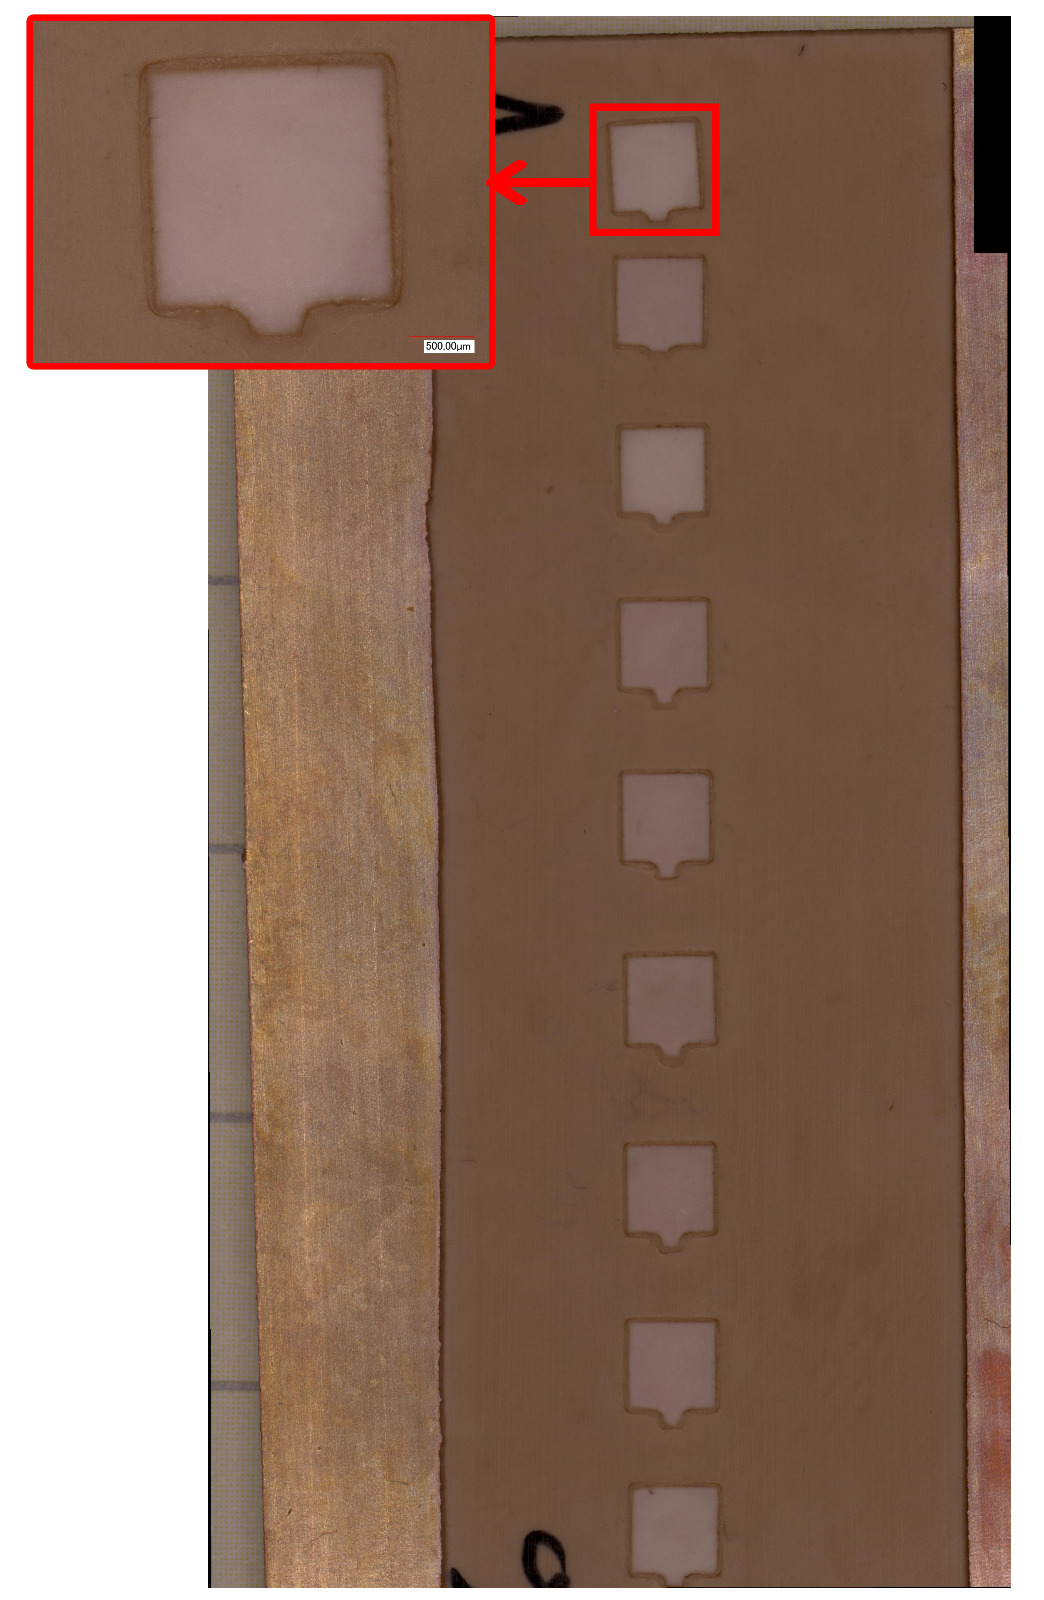
\includegraphics[scale=0.2]{Bilder/WhatsApp Image 2025-03-28 at 21.29.51.jpeg}
    \caption{Bruchanalyse laminiert hergestellter Scherkörper mit Kupferbodenplatte, (Selbsterstellte Abbildungen)}
    \label{lamWhats}
\end{figure}

Die Analyse der Bruchmuster gesinterter Scherkörper zeigt, dass durchgängig ein Mischungsbruch innerhalb der Fügepartner 2 und 3 vorliegt. Charakteristisch hierfür ist das partielle Verbleiben von Fügepartner 2 (Silber) auf der Oberfläche von Fügepartner 3 nach dem Schertest. Eine Ausnahme bildet Prüfkörper 7, bei dem nahezu der gesamte verbleibende Materialanteil Fügepartner 2 zuzuordnen ist, was auf eine veränderte Bruchmechanik in diesem spezifischen Fall hindeutet. (siehe \hyperref[sin]{Abbildung 7})

\begin{figure}[H]
    \centering
    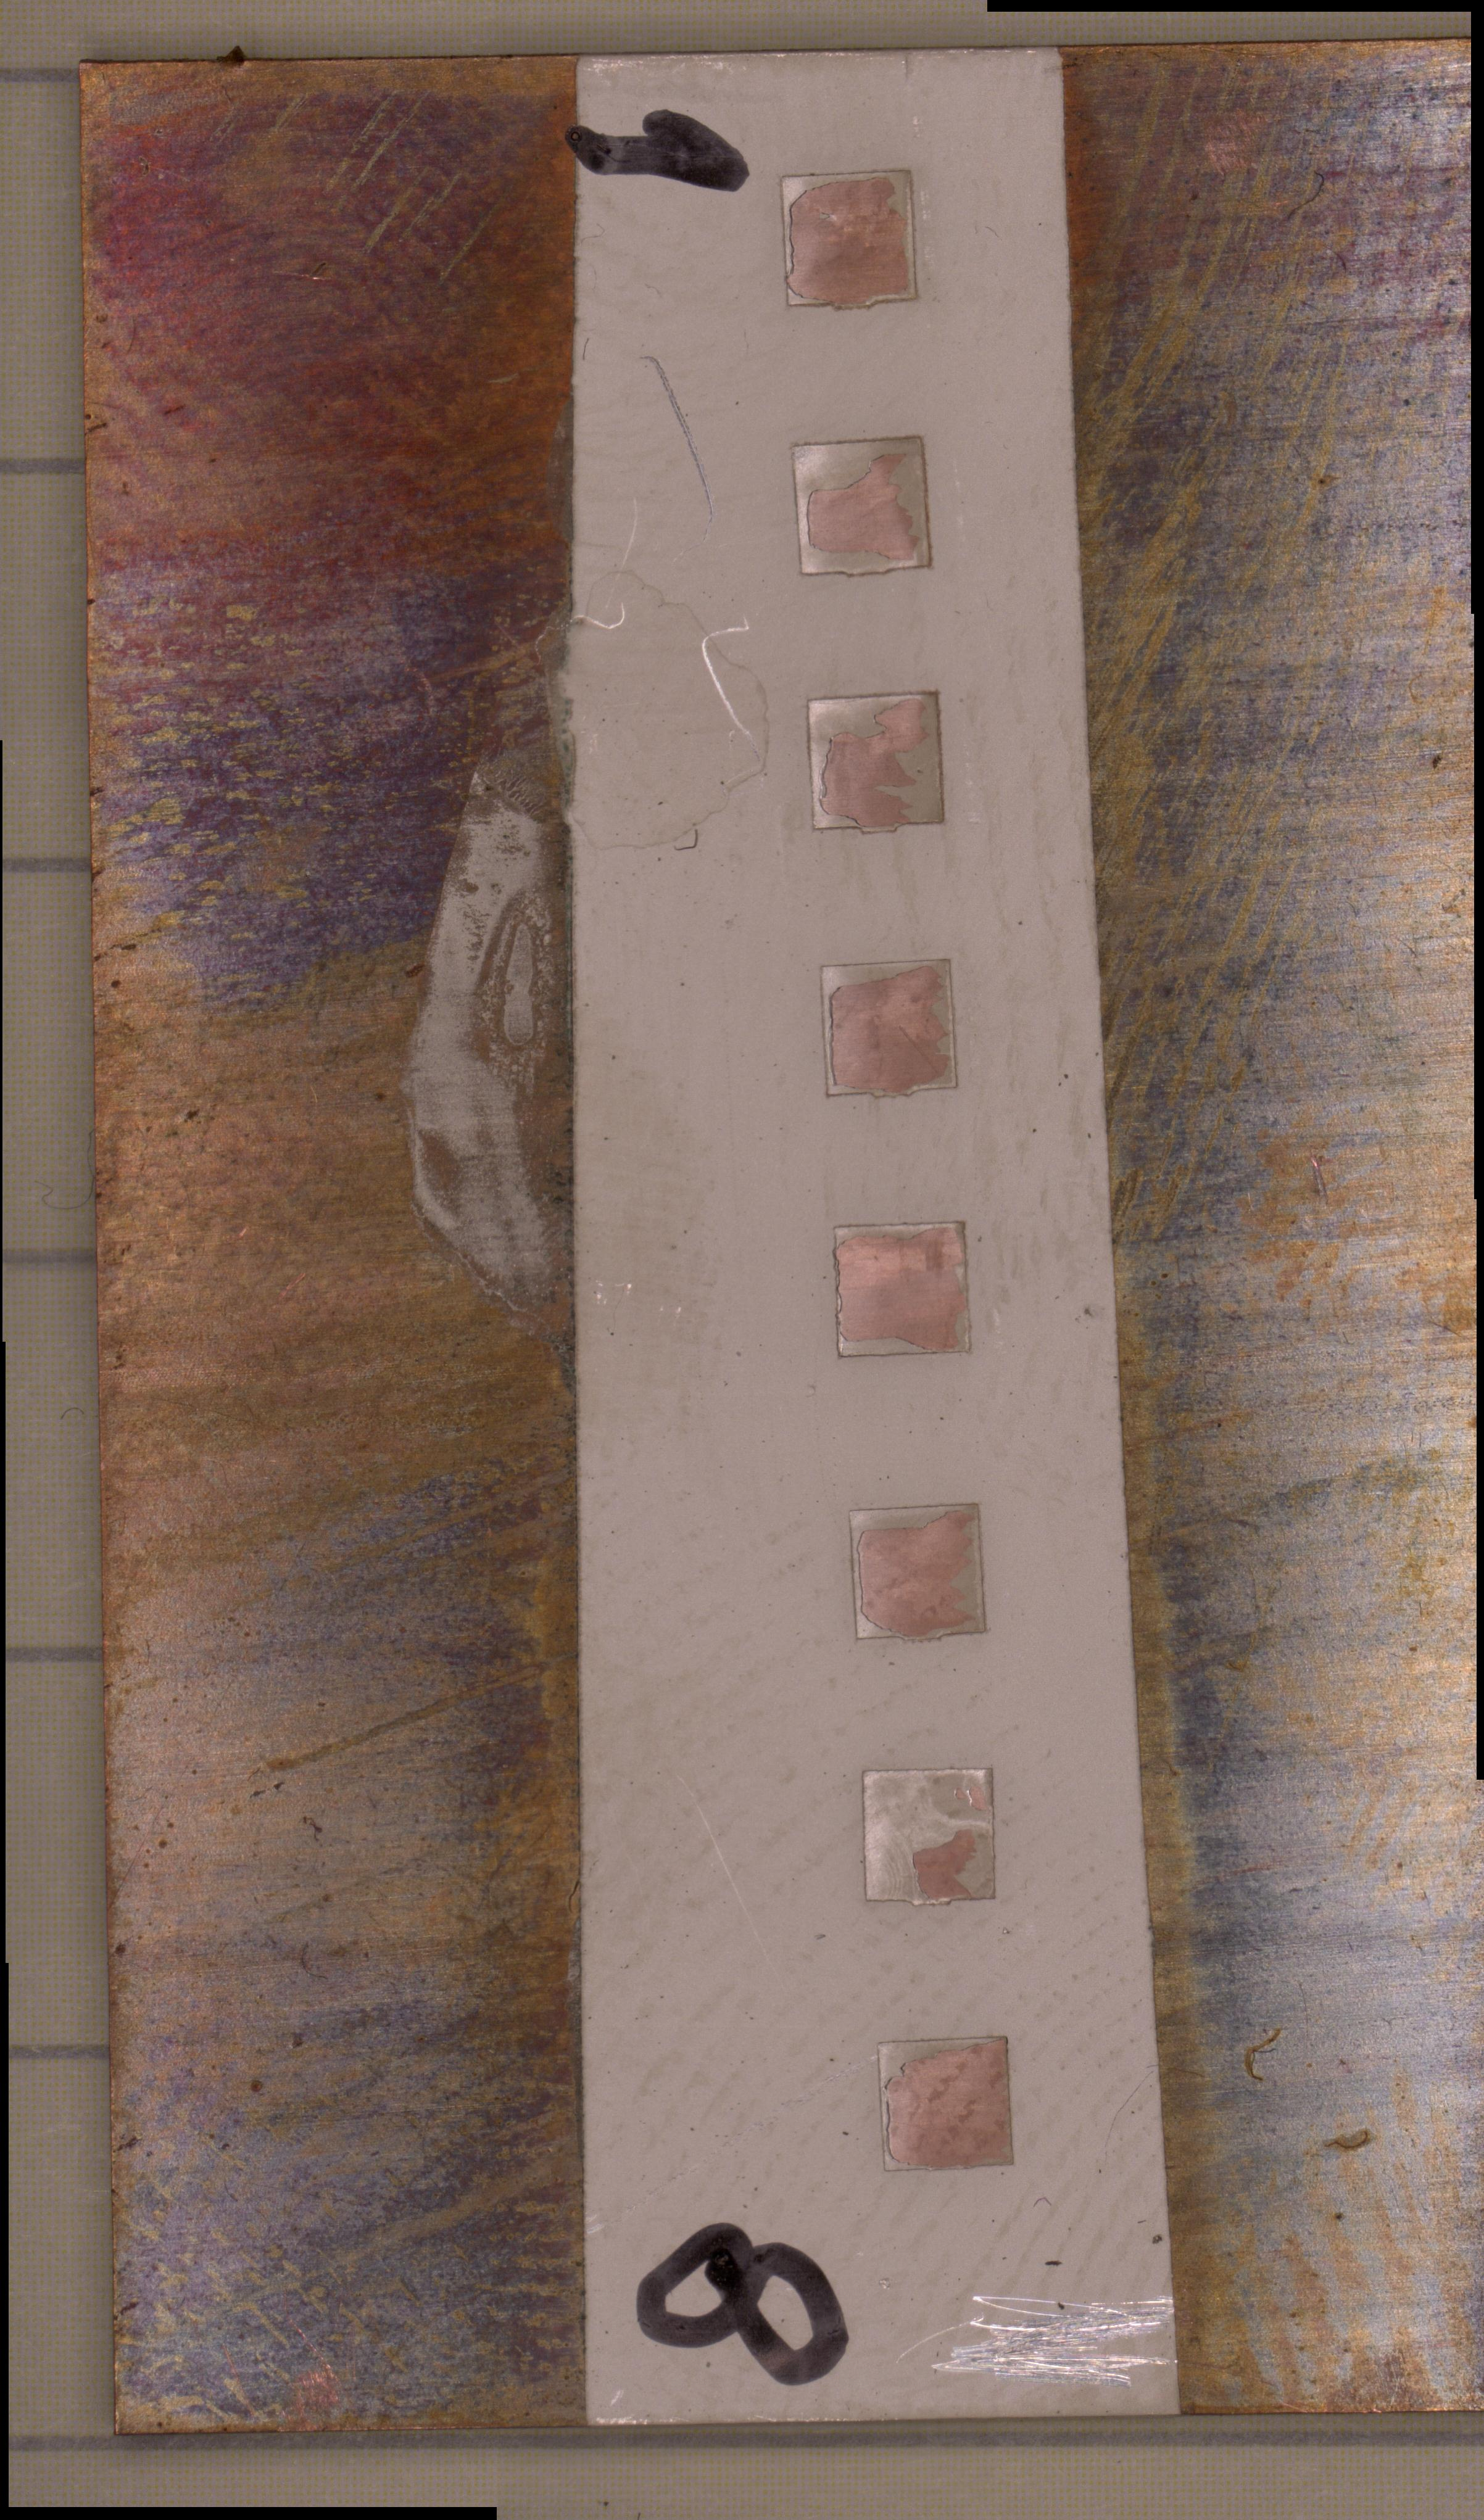
\includegraphics[scale=0.07]{Bilder/Bodenplatte_Sintern_Gesamt.jpg}
    \caption{Bruchanalyse gesintert hergestellter Scherkörper mit Kupferbodenplatte, (Selbsterstellte Abbildungen)}
    \label{sin}
\end{figure}

Mikroskopische Nahaufnahme von Prüfkörper 2 im Bereich der Fügezone. Deutlich erkennbar ist, dass der Großteil des Fügepartners 2 nach dem Schertest entfernt wurde und auf dem Prüfkörper verblieben ist, wodurch der darunterliegende Fügepartner 3 sichtbar wird. (siehe \hyperref[sin2]{Abbildung 8})

\begin{figure}[H]
    \centering
    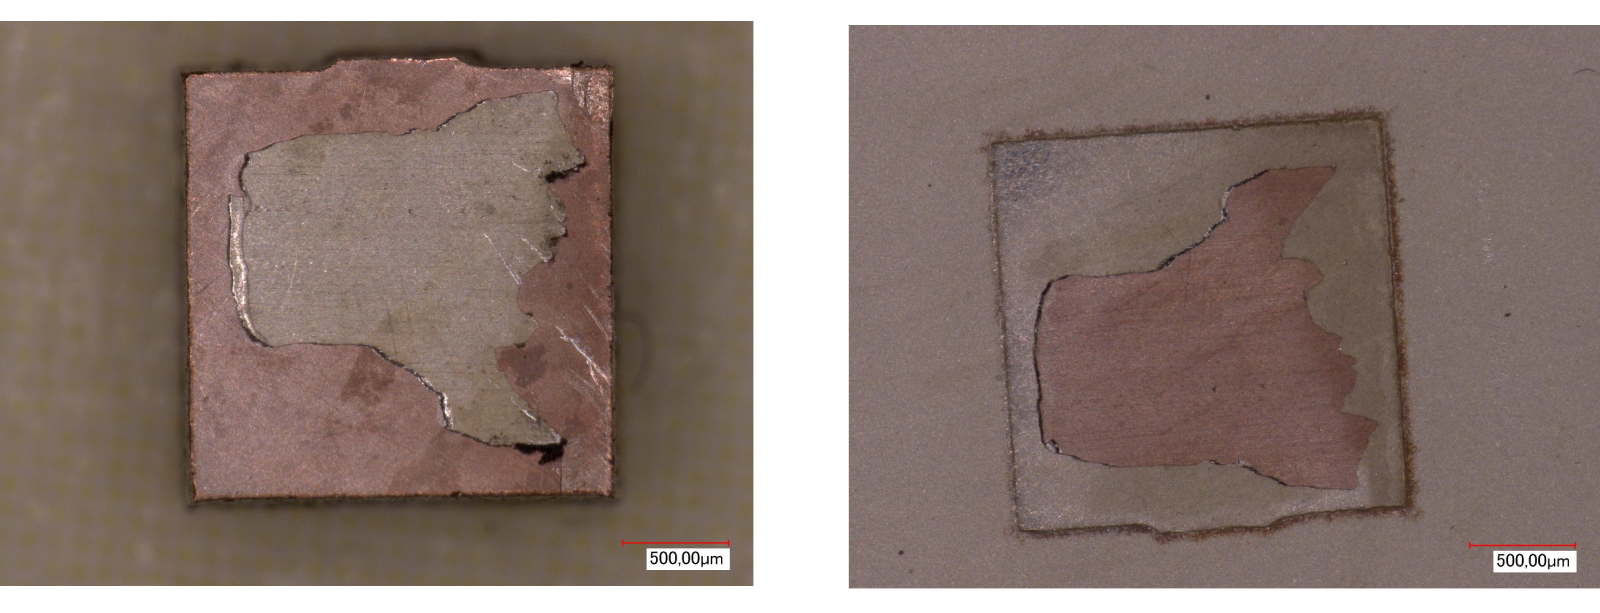
\includegraphics[scale=0.2]{Bilder/2s.png}
    \caption{Mikroskopische Aufnahme von Prüfkörper 2 und Kupferbodenplatte nach dem Schertest (gesintert), (Selbsterstellte Abbildungen)}
    \label{sin2}
\end{figure}

Mikroskopische Nahaufnahme von Prüfkörper 7 mit Mischungsbruch, bei dem ein größerer Anteil von Fügepartner 2 auf der Bodenplatte verbleibt als bei den anderen Prüfkörpern. (siehe \hyperref[sin7]{Abbildung 9})

\begin{figure}[H]
    \centering
    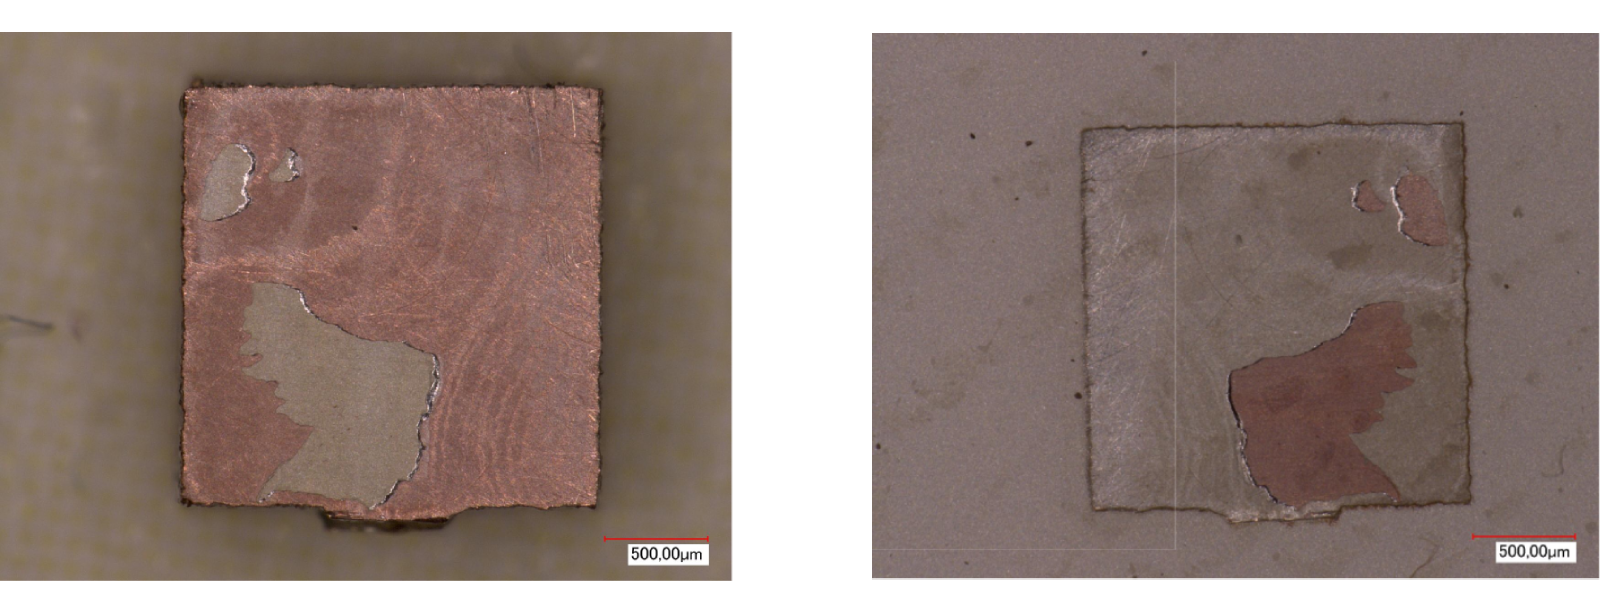
\includegraphics[scale=0.2]{Bilder/7s.png}
    \caption{Prüfkörper 7 und Kupferbodenplatte nach dem Schertest (gesintert), (Selbsterstellte Abbildungen)}
    \label{sin7}
\end{figure}

Nach der qualitativen Analyse der Bruchmuster folgt die quantitative Auswertung der Scherfestigkeiten anhand eines Boxplots. Die gemessenen Werte verdeutlichen signifikante Unterschiede zwischen den beiden Herstellungsverfahren.\\

Die gesinterten Prüfkörper weisen insgesamt höhere Scherfestigkeitswerte auf, wobei sowohl der Median als auch das obere Quartil deutlich über denen der laminierten Proben liegen. Dies bestätigt die zuvor beobachteten Bruchmechanismen und unterstreicht die höhere mechanische Belastbarkeit gesinterter Verbindungen. Die vergleichsweise breite Streuung der Messwerte bei den gesinterten Prüfkörpern deutet jedoch darauf hin, dass individuelle Materialeigenschaften oder prozesstechnische Schwankungen eine Rolle spielen könnten.\\

Die laminierten Prüfkörper zeigen hingegen eine deutlich engere Verteilung mit durchgängig niedrigeren Scherfestigkeiten. Dies steht im Einklang mit den beobachteten Adhäsionsbrüchen und lässt auf eine geringere Haftfestigkeit innerhalb der Grenzschicht schließen. Da die Variabilität der Werte hier geringer ist, kann davon ausgegangen werden, dass das Laminierungsverfahren reproduzierbar, aber grundsätzlich mechanisch unterlegen ist.\\

Die Kombination aus qualitativer Bruchbildanalyse und quantitativer Auswertung der Scherfestigkeiten liefert somit ein umfassendes Bild der mechanischen Eigenschaften beider Herstellungsverfahren. Die Ergebnisse belegen die Überlegenheit des Sinterverfahrens hinsichtlich der erzielbaren Scherfestigkeit, während gleichzeitig die Variabilität innerhalb der gesinterten Proben auf potenzielle Optimierungsmöglichkeiten im Herstellungsprozess hinweist.

\begin{figure}[H]
    \centering
    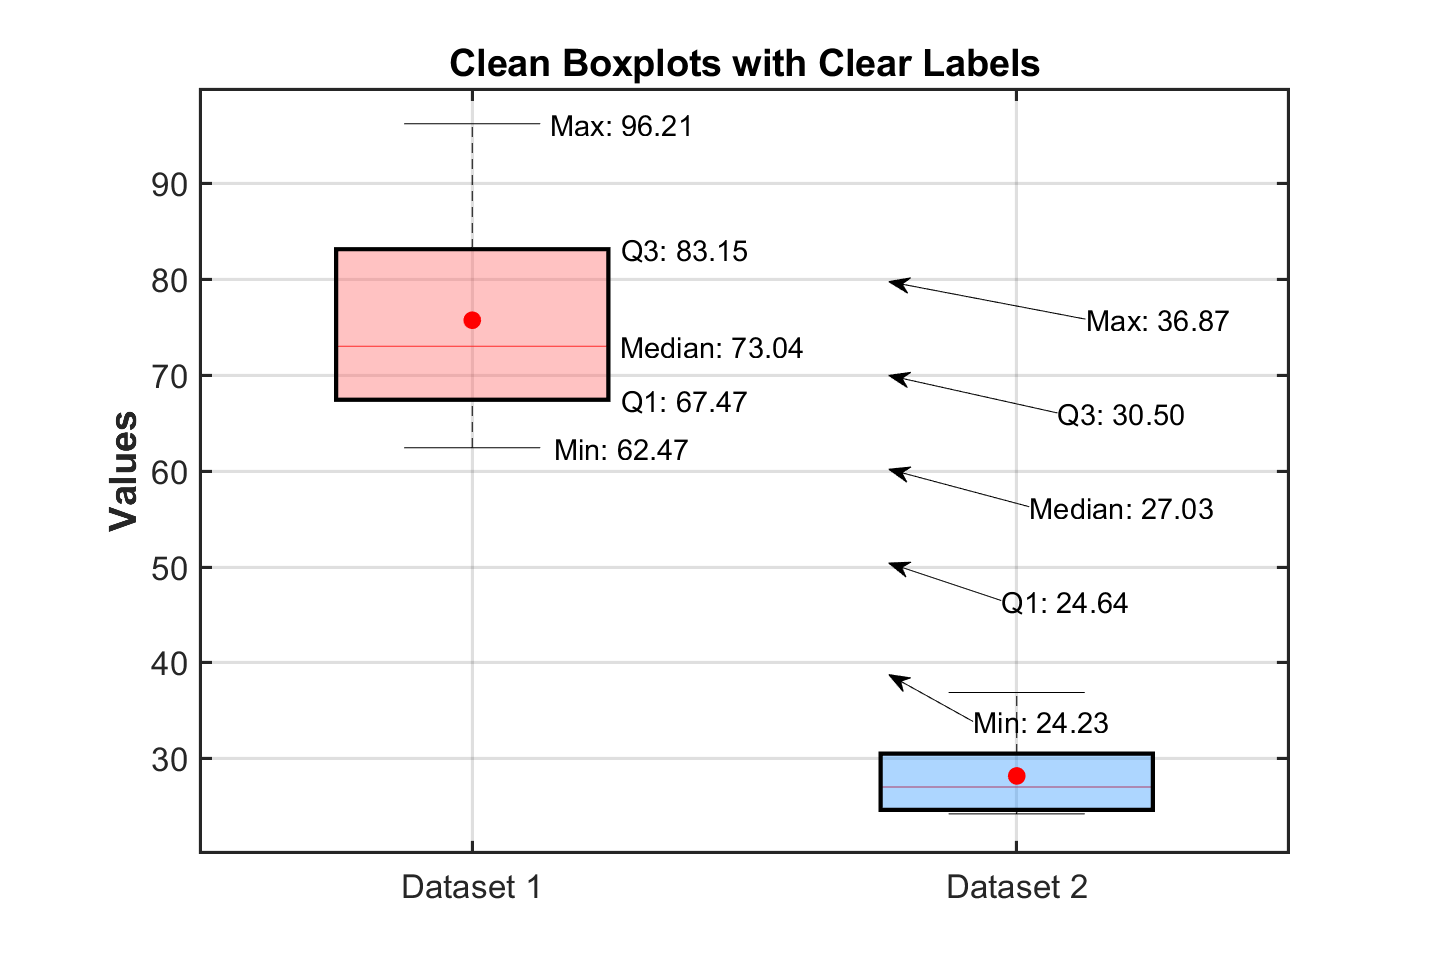
\includegraphics[width=0.7\textwidth]{Bilder/boxplot_final.eps}
    \caption{Boxplot der Scherfestigkeit {[}N/mm$^2${]} von gesinterten und laminierten Scherkörpern.}
    \label{fig:boxplot}
\end{figure}




